\chapter{プログラミング言語Swift}
\label{explain-swift}

本章では、本研究の対象であるプログラミング言語Swiftの言語的特徴とSwiftコンパイラの構成について述べる。

\section{Swiftの特徴}
\label{explain-swift:features}

~\ref{explain-bootstrap:merit}節および~\ref{explain-bootstrap:issue}節で述べたように、Swiftは他の言語と比較しても多くの特徴を備えており、それがこのコンパイラの複雑性を増しているためにBootstrapにおける費用対効果の試算を困難にする原因となっている。

本節ではそうしたSwiftの特徴について概説する。

\subsection{マルチパラダイム}

プログラミング言語が採用するプログラミングパラダイムによって、その言語のコンパイラの設計、特に構文解析器とコード生成部分の設計は大きな影響を受ける。
Swiftは近年の汎用言語に採用されている多くのプログラミングパラダイムを取り入れているマルチパラダイムプログラミング言語であり、以下のようなプログラミングパラダイムを採用している。

\subsubsection{関数型プログラミング}

Swiftでは関数を第一級のオブジェクトとして扱い、2つの型から成る関数型を用意することで、MLやHaskellなどの言語と同様のラムダ計算に近しい表記方法を行う関数型プログラミングが可能となっている。

Swiftにおける関数型プログラミングの例をプログラム~\ref{code:functional}に挙げる。
関数用の型が矢印演算子によって提供されており、関数自体を変数に代入して使用できていることがわかるだろう。

\begin{lstlisting}[caption=Swiftにおける関数型プログラミングの例, label=code:functional]
let f: Int -> Int = { x in x + 1 }
print(f(1)) // 標準出力に 2 と表示する
\end{lstlisting}

このパラダイムにより、コンパイラではCやJava、C++と比較して関数のために無名関数や部分適用といったより多くの構文を用意し、一般的に関数を第一級オブジェクトとして扱わない事が多いアセンブリ言語へは関数ポインタなどを使用することでそれらの構文を翻訳する必要がある。

\subsubsection{オブジェクト指向プログラミング}

Swiftが提供する複合型であるクラス、構造体、列挙体、プロトコルでは継承関係を定義することができ、外部の手続きから呼び出し可能な値や他の型定義などのメンバを持つことができるように設計されていることで、オブジェクト指向プログラミングを可能としている。

Swiftにおけるオブジェクト指向プログラミングの例をプログラム~\ref{code:objective}に挙げる。
この例では継承関係のあるクラスから生成されたオブジェクトに対し、クラスで定義された関数のメンバを呼び出している。

\begin{lstlisting}[caption=Swiftにおけるオブジェクト指向プログラミングの例, label=code:objective]
class Parent {
    func f() { print("parent") }
}

class Child : Parent {
    override func f() { print("child") }
}

let x: Parent = Child()
x.f() // 標準出力に child と表示する
\end{lstlisting}

このパラダイムを実現するために、コンパイラでは各複合型ごとのスコープの管理が必要になり、継承関係のある型同士を部分型として扱った上で、仮想関数テーブルなどを用いて実行時に呼び出すメンバを動的に決定できる仕組みを生成する必要がある。

\subsubsection{パターンマッチ}

Swiftは特定の構造を持つ値についてその一般的なパターンを定義し、変数を含む左辺値と変数を含まない右辺値を比較することで左辺値中の変数の型と値を決定するパターンマッチの機構を持っている。

Swiftにおけるパターンマッチの例をプログラム~\ref{code:pattern-match}に挙げる。
現在のSwiftではこの例内の6行目のような列挙体やタプルの値について特に柔軟なパターンマッチを提供している。

\begin{lstlisting}[caption=Swiftにおけるパターンマッチの例, label=code:pattern-match]
enum Sample {
    case X, Y(Int)
}
let x = Sample.Y(1)

if case Sample.Y(let v) = x {
    print(v) // 標準出力に 1 と表示する
}
\end{lstlisting}

このパラダイムの実現には、コンパイラで左辺値のパターンが表す構造と型を解釈し、右辺値の値をより詳細な構造に分解してより単純な同値性を確認する演算や変数の宣言の集まりに変換する必要がある。


\subsection{強力な型システム}

強力な型システムはプログラマのミスを発見する有効な手立てとなり得るが、一般的にコンパイラの型推論や型検査にかかる時間との間でトレードオフの関係となる。
以下ではSwiftで採用されている型システムの特徴について述べる。

\subsubsection{型パラメータ多相}

Swiftでは各複合型や関数内で用いられている型を全称型を持つ変数で記述することにより、複数の型を対象とした複合型や関数を記述できる型パラメータ多相を採用している。

コンパイラでは全称型を持つ複合型や関数をその文脈によって決定された型で具体的に定義しなおし、それらの具体的に定義された型を同一の型として扱う必要がある。
この機能の実装は後述する型推論において型の解決が可能かどうかを決定するためのステップを大幅に増加させてしまうため、コンパイル時間との兼ね合いを考えてより絞り込んだ制約を要求するなど、状況に合わせたサポート機能の組み込みが要求される。

\subsubsection{関数のオーバーロード}

Swiftは引数の数が異なる関数や引数の型が異なる関数を同じ名前で定義できる、関数のオーバーロード機能を有している。

この機能によってコンパイラでは、どの関数が呼びだされているかを決定する前にその関数の型を決定するステップを追加しなければならなくなる。
ただし、型推論による型の決定には関連する項の参照が解決されて型注釈などが把握されている必要があるため、関数呼び出し以外の項については型を決定する前に参照を解決する必要があり、オーバーロードの機能を追加すると関数呼び出しと他の項を同一の手順で参照解決・型解決できなくなるという複雑性を含まざるを得なくなる。

\subsubsection{型推論}

Swiftでは関数型プログラミングを可能とする多くの言語と同様にHindlyとMilnerによるアルゴリズムを採用した強力な型推論を備えている。

HindlyとMilnerによるアルゴリズムはMLやHaskellなど多くの関数型プログラミングを採用する言語で採用されているが、前述のとおりオブジェクト指向や型パラメータ多相、関数のオーバーロードを許すという特徴から、Swiftコンパイラではそれを大きく拡張した形で実装しなくてはならない。


\subsection{高い可読性}
\label{explain-swift:features:readability}

Swiftがマルチパラダイム性と強力な型システムの他にその言語の特徴として大きく掲げているのが、高い可読性である。
Swiftでは未定義値を安全に取り扱うためのオプショナル型や無名関数を定義するためのクロージャ、複数の値をまとめて扱えるタプル、自由なデータ構造を記述可能な列挙体などについてその可読性を高めるための糖衣構文を用意している。

また、糖衣構文などを提供するために構文の曖昧性を残しているのもSwiftの特徴である。
例えば、プログラム~\ref{code:ambiguous}のような構文はSwiftの構文定義に則った全く正しいコードだが、一般的なアプローチでは正しく解析することができない。
xの後に続く\{がxの引数のクロージャの始まりなのかif文の本体の始まりなのかは、xが引数としてクロージャを取る関数であることを解析機が知っていなければ決定できず、かつそのxはこれから解析を行う他のファイルなどに宣言されている可能性があるために、全てのファイルの解析を完了するまでxの参照を解決することはできない可能性があるためである。

\begin{lstlisting}[caption=曖昧な構文を持った正しいSwiftコード, label=code:ambiguous]
let x: (() -> ()) -> Bool = { f in true }

if x { print("closure") } { print("if") }
\end{lstlisting}

こうした構文を一切の曖昧性なしに解析するためにはコンパイル対象となるプログラムを参照の解決に必要な回数だけ走査しなくてはならなくなるが、それは少なく見積もっても大変非効率であり、現実的ではない。
現状のSwiftコンパイラではこうした曖昧な構文は可能性のあるどちらかの構文に決め打ちして実装されており、もう一方を意図して記述しているプログラマに対しては全く見当はずれのエラーメッセージを提示することとなっている。


\section{Swiftコンパイラの構成}
\label{explain-swift:structure}

~\ref{explain-swift:features}節で述べた特徴を実現するために、Swiftコンパイラではその詳細な設計において多くの工夫が行われている。
本節ではその詳細な工夫について本研究で評価の対象としている構文解析器のみについて説明し、その他の箇所については概要を述べるだけに留める。

\subsection{Swiftコンパイラの概要}

Swiftコンパイラは大まかに図~\ref{img:swift-compile-process}のような構造を持つ~\cite{sil}。
% TODO 図の差し替えと詳説

\begin{figure}
    \begin{center}
        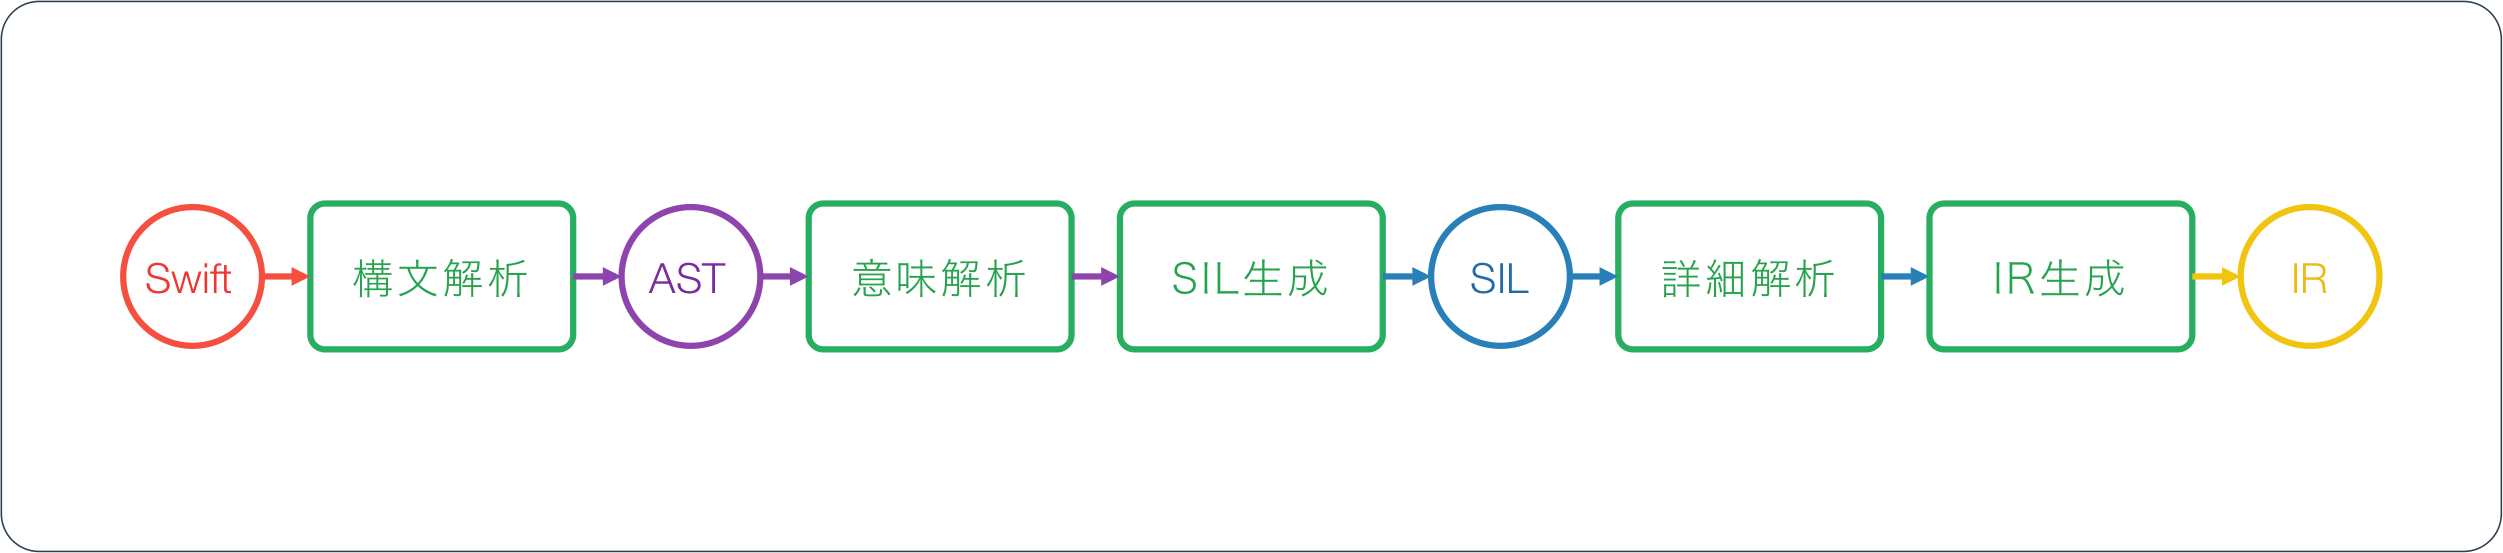
\includegraphics[scale=0.30]{./img/swift_compile_process}
        \caption{Swiftコンパイラの構成}
        \label{img:swift-compile-process}
    \end{center}
\end{figure}

構文解析の詳細については~\ref{explain-swift:structure:parser}節で詳しく述べるが、Swiftコンパイラは構文解析時に可能な限り変数や型などの参照を解決し、続く意味解析で不明だった参照の解決と明示されていない型の推論、型の整合性の検査を行う。

また、コンパイラの構成で特に特徴的なのは意味解析とLLVM-IRのコード生成との間にSIL(Swift Intermediate Language)という独自の中間表現を挟んでいる点である。
Swiftコンパイラでは、このSIL形式でAST(Abstruct Syntax Tree)では解析しづらいコールグラフやクラス階層に基づくエラーの検出やメモリ管理用コードの挿入、最適化などを行っている。

SIL形式が複雑な解析部分を担っているためにSwiftコンパイラの構文解析器とASTは意味解析より後のステップで更に改変されること無く、完全に分離されている。
そのため、コンパイラ中の構文解析部分のみを抽出して他の実装と比較評価を行うことが可能となっている。


\subsection{Swiftコンパイラの構文解析器}
\label{explain-swift:structure:parser}

~\ref{explain-swift:features}節で述べたようにSwiftは多くの特徴を持っているため、その構文は他の言語と比較しても複雑なものとなっており、構文解析には高い柔軟性が求められる。
以下ではSwiftコンパイラの構文解析器における各機能についてその特徴を述べる。

% TODO 字句解析

\subsubsection{LL(k)方式構文解析}

現行のSwiftコンパイラでは再帰下降構文解析の一種であるLL(k)方式を構文解析に採用しており、その構文解析器はC++の関数として書き下されている。

LL(k)方式では解析する対象の構文によって解析器が先読みを行うトークンの数を変更することで、各構文に必要な先読みの数を最小限に抑えながらも、~\ref{explain-swift:features:readability}節で取り上げたような完全な曖昧性を持つ構文以外は必ず解析対象の構文を決定することができる。

また、単なるLL(k)方式の構文解析器が自動生成が可能であることは~\cite{antlr}などで知られているが、Swiftの場合は先述の曖昧な構文に対する対処やより詳細なエラーの報告を行うために、構文解析器を全て手動で書き下している。

\subsubsection{参照解決}

現行のSwiftコンパイラでは構文解析時に可能な限り変数や型の参照を解決し、他のファイルで宣言されている可能性のあるものなど、その時点で解決不可能なものについては解決不可能としてマークしてASTに組み入れる。
解決が不可能であった参照は全てのファイルを走査し終えた後の意味解析の最初のステップで解決される。

% TODO スコープ解決、メンバ呼び出し

\subsubsection{AST}

% TODO 型情報の保持方法、ASTの展開方法

\subsubsection{曖昧な構文の解析}

Swiftコンパイラの構文解析器では、構文定義的に参照の解決などが行われた後でなければどの構文なのかを判断することができない曖昧な構文については、ひとまず特定の構文として解析して意味解析時に適切な形式でなかった場合にのみそれを変換する。

%%% Local Variables:
%%% mode: japanese-latex
%%% TeX-master: "../thesis"
%%% End:
